% sage_latex_guidelines.tex V1.20, 14 January 2017

\documentclass[Crown,sagev,times]{sagej}

\usepackage{moreverb,url}
\usepackage{graphicx}
\usepackage{subcaption}
\usepackage{soul}
\usepackage{natbib}
\usepackage[colorlinks,bookmarksopen,bookmarksnumbered,citecolor=red,urlcolor=red]{hyperref}

\bibliographystyle{SageV}


\newcommand\BibTeX{{\rmfamily B\kern-.05em \textsc{i\kern-.025em b}\kern-.08em
T\kern-.1667em\lower.7ex\hbox{E}\kern-.125emX}}

\def\volumeyear{2016}

\begin{document}
\title{You change the way you talk:
Examining the network, toxicity, and discourse
of cross-platform users on Twitter and Parler
during the 2020 U.S. Presidential Election}

\author{Anonymous Authors(s)\affilnum{1}}
\affiliation{\affilnum{1}Anonymous Institution(s)}
\corrauth{Anonymous Author(s)}
\email{anonymous@sage.co.uk}

\begin{abstract}
This study examines code-switching behaviors of cross-platform social media users specifically between Twitter and Parler
during the 2020 U.S. Presidential Election. Utilizing social identity theory as a framework, we examine messages related to voter fraud by 
users who migrated from Twitter to Parler following Twitter bans. Our analysis covers 38,798 accounts active on both platforms, 
analyzing 1.5 million tweets and more than 100 thousand parleys. The key findings of the study are as follows: 
First, we discovered differing levels of network homophily between high degree centrality and low degree centrality cross-platform users, 
illustrating how individuals with varying degrees of influence engage differently across platforms. Second, we observed higher toxicity levels 
in heterogeneous networks, which include both in-group and out-group members, compared to homogeneous networks that are primarily composed of in-group members. 
This suggests the level of toxicity in online spaces correlates with the level of group diversity. 
Third, we found that cross-platform users created distinctive discourse community with in-group and out-group members, 
indicating that content and discussions within these networks are influenced by the social identity dynamics of the users. 
Our study contributes to the current research in political communication and information science by proposing comparative user analyses across multiple social media platforms. 
Focusing on a critical period of platform transition during a contentious political event, our study offers insights into the dynamics of online communities 
and the shifting nature of political language used by social media users.
\end{abstract}

\keywords{Network analysis; code-switching; toxicity; political discourse; social media; Twitter; Parler; cross-platform analysis; alternative social media}

\maketitle

\section{Introduction} \label{sec:intro}

Social media have emerged as a key platform for sharing opinions and exchanging information, leading some scholars to suggest that 
it might actualize the Habermasian idea of the public sphere--the ideal discursive space where citizens can engage in rational debate 
free from the influence of societal political and economic powers and form their opinions independently \cite{Bruns2015,Benkler2006, habermas1991structural}.
Similar to this projection, social media have shown a potential that it could become a place where users express their views toward certain issues 
\cite{ocal2021reasoning} with little intervention from the platform moderators or authorities \cite{gibbs2013overcoming}. 
However, the openness and lack of regulations on social media have also led to unwanted byproducts such as incivility, mis/disinformation, 
and political polarization. In addition, social identity theory suggests that individuals tend to gravitate towards others who share their views 
while showing bias against those with opposing opinions \cite{tajfel1979integrative}. This tendency fuels the creation of partisan echo chambers 
on social media, where misinformation can spread unchecked among like-minded users and hamper meaningful democratic discourse 
across different viewpoints \cite{sunstein2018republic, grevet2014managing}. 
This identity-based fragmentation on social media is of particular concern in the context of the rising importance of identity politics 
in contemporary political discourse \cite{Cramer2016}.

Research has examined how the level of homogeneity in the network is related to the way people share 
political information with other members of online social networks \cite{gibbs2013overcoming, Conover2011}, 
however, the majority have focused exclusively on a single platform. One of the most reasonable explanations 
for the popularity of single-platform research is related to data availability. Due to the complex governance of social media platforms, 
each platform has different levels of data-sharing policy for researchers. For instance, Twitter used to provide Academic APIs 
to allow researchers to collect large amounts of data for research purposes whereas Facebook provides more limited access to its data. 
This gap naturally led researchers to use Twitter data more frequently because the data are considered a low-hanging fruit. 
Another reason for the predominance of single-platform research is related to the diversity of platform affordances. 
Different affordance characteristics offered by various platforms often called the multi-modality of data 
(e.g., texts from Twitter vs. videos from TikTok) require unique analytical strategies that often complicate the analysis using data from multiple platforms.

However, focusing only on a single social media platform for user analysis can limit our ability to gain a comprehensive understanding of 
how the same user may communicate differently when they communicate across multiple platforms, each with varying levels of network homophily, 
distinct social norms, and specific content regulation policies.
To address the gap, this study takes a multi-platform approach. We focus on two social media platforms that were highly relevant to 
voter fraud claims during the 2020 U.S. Presidential Election campaigns: Twitter and Parler. By comparing the communication patterns 
of the users who have accounts on both platforms, we aim to answer questions regarding 
(1) the difference in the network structure of cross-platform users, 
(2) the effects of network homogeneity on the way people communicate toxic language with in-group and out-group members
, and (3) the types of information shared in different social media platforms.

\subsection{Context of the study}

During the 2020 U.S. Presidential Election, then-President Trump and his campaign alleged that mail-in ballots were likely to be fraudulent and actively spread these claims across popular social media platforms \cite{lima2020}. As part of their effort to combat misinformation, Twitter decided to suspend any accounts that were involved in disseminating voter fraud claims \cite{twitter2021}, including the account of President Trump. In response to Twitter's action, numerous users migrated from Twitter to alternative social media platforms. This course of migration was a collective action of the users who felt not just constrained but also alienated from the community, especially when they perceived an increase in censorship \cite{kiene2016surviving}. Many of the users who left Twitter found a safe haven in Parler, an alternative social media platform that proclaimed that they allow users to ``speak(s) freely and express yourself openly, without fear of being de-platformed for your views.'' As a result, Parler has gained attention from conservatives who were looking for alternative social media that would accept them for who they are \cite{pewresearch}.
Parler was also known to be one of the main social media that were actively used to organize the January 6 Capitol attack. 
This provides a unique opportunity to compare the cross-platform behaviors of individual users and identify differences in communication patterns. 
Comparing language use between platforms such as Twitter and Parler offers a relatively equitable comparison due to similarities 
in their affordances \cite{bucher2018affordances}. This allows for a thorough analysis of these differences \cite{m2021political}. 
To examine these questions further, we propose the following research questions.

 \subsection{Research Questions and Major Findings}

\begin{itemize}
    \item RQ 1: How do cross-platform users form network structures for in-group and out-group communication?
    \item RQ 2: Do the toxicity levels of conversations vary between interactions with in-group members and out-group members?
    \item RQ 3: Do cross-platform users share different information when they communicate with in-group members versus when they communicate with out-group members?
\end{itemize}

The main findings of this study can be summarized as follows: 

 \begin{itemize}
     \item Finding 1: There are varying degrees of homophily among cross-platform users. Cross-platform users with high degree centrality exhibit a higher level of heterophily (communication with out-group members) compared to cross-platform users with lower degree centrality, who tend to communicate more with in-group members. 
     \item Finding 2: The level of toxicity in out-group communication is higher than the level of toxicity in in-group communication. This finding aligns with previous scholarship on group communication theory, which found that in-group relationships tend to be more congenial than out-group relationships.
    \item Finding 3: Information shared by cross-platform users on Twitter and Parler differs, creating distinct discourses on each platform. This finding suggests that varying levels of network homogeneity across these platforms can influence the types of information people choose to share or withhold on specific platforms.
 \end{itemize}

For transparency and reproducibility, we have made our code publicly available at \url{https://github.com/park-jay/cross-platform}. 

\section{Related Works} \label{sec:related_works}
\subsection{Echo chambers in social media} \label{sec:echo_chambers}

Group polarization theory suggests that echo chambers can lead partisans to hold their existing views more strongly when they are exposed only to opinions from their own side, thus intensifying their political dispositions. Social media provide a platform for like-minded partisans to connect and create echo chambers \cite{sunstein2018republic}. These online echo chambers not only foster tribal mindsets and exacerbate attitude polarization among the public \cite{gillani2018me}, but also function as a communication space for hate speech \cite{zannettou2018gab}. Moreover, echo chambers hinder people from sharing perspectives with members of out-groups\cite{dori2021restoring}.
Existing research has explored echo chambers on social media by comparing the prevalence of hate speech in comments on the social media accounts of traditional media outlets. A study analyzing user comments on news coverage of the 2020 U.S. Presidential Election found that the comments on liberal (CNN) and conservative (Fox News) media exhibit different trolling styles across social media platforms (e.g., Twitter, Facebook, and Instagram) and between media channels \cite{fichman2023trolling}. Another study on the January 6th Capitol attack revealed a significant presence of hate speech on Twitter, particularly targeting Republican politicians and women \cite{kim2022violent}. 
While legacy and mainstream social media platforms implement moderation processes to mitigate hate speech on the platform, researchers found that fringe social media platforms, which tolerate extreme views to protect the ``free speech'' rights, tend to lack content moderation policy, thus allowing more hate speech. 

For instance, Gab, a far right-leaning social media platform, gained attention from users seeking an alternative social media platform with minimum content moderation policy in the name of protecting the right of free speech \cite{fair2019shouting}.  
Mathew et al. examined how fast hateful content can travel inside Gab and be delivered to non-hateful users \cite{mathew2019spread}. They found that more hateful content diffuses faster and farther in the network compared to the content generated by normal non-hateful users.
Another study argues that Gab attracts alt-right users, conspiracy theorists, and other trolls \cite{zannettou2018gab}.
However, despite the potential harm of online echo chambers on fringe social media platforms, there is currently a lack of research comparing their characteristics with those of mainstream social media and how these characteristics related to the information shared on them. Our study examines Parler, a fringe social media platform accused of enabling hate groups to organize and strategize before and during the U.S. Capitol attack on January 6th, 2021, and compares it with Twitter. This approach aims to enrich the scholarship on fringe online social media studies by introducing a multi-platform perspective. 

\subsection{Toxic political discourse} \label{sec:affective_polarization}
The proliferation of echo chambers on social media poses challenges that can strain the democratic underpinnings of the society in many ways. In particular, affective polarization, characterized by a deeply connected emotional attachment to one's political views and identity, is one of the main factors that exacerbate the existing political division of society \cite{iyengar2012affect}. Heightened affective polarization might lead people to actively evade contrasting viewpoints, seeing opposing views as not only inaccurate but also as immoral or even dangerous \cite{mutz2018status, prior2005news}. 
Increasing levels of affective polarization also have been associated with the erosion of constructive political debate, inter-party cooperation, and a decline in willingness to accept electoral defeat \cite{iyengar2019origins}. Additionally, there is an observable bias toward supporting political extremism as people increasingly distance themselves from opposing political groups. Such distancing can lead to the use of negative language and stereotypes towards the opposition \cite{kalmoe2019lethal}.
We argue that the relationship between affective polarization and toxic discourse on social media is evident and concerning. To understand its democratic implications, we focus on social media, the critical arena of toxic discourse, as Kubin and Von Sikorski’s review of affective polarization found that nearly all experiments showed that social media increase people’s polarization \cite{kubin2021role}.
Existing evidence suggests that those who are more polarized use more toxic language when addressing members of the opposite political spectrum on these platforms \cite{barbera2015understanding}. However, there is little research that examines whether people change the style of discourse (e.g., the amount of toxic language use) when there are more or less like-minded others on the platform; thus, more research is needed on this topic. 

\subsection{In-/out-group communication and code switching} \label{sec:in_out_group}

In early works on in-group and out-group communication, Sumner described that people associate peace with in-groups while associating hostility and war with out-groups \cite{sumner1906folkways} . 
In the same way, people tend to find the language within in-groups to be more favorable than that of out-groups \cite{tong1999language}. 
According to social identity theory, individuals do not think of themselves as ``distinctive packages of traits'' but instead as parts of larger cultural and socioeconomic groups and have an inherent bias of dividing ``us'' from ``them'', viewing members of our in-groups as more favorable than out-group members \cite{tajfel1979integrative}. 

People also tend to shift their linguistic styles based on who they are communicating with. An et al.'s study of user behavior on social media found that users exhibited different linguistic styles when they were in a homogenous communication space (only in-group members) from when they were in a space with a diverse group of people \cite{an2019political}. 
Taken together, the affective polarization and social identity research shows that partisans' worldviews are instinctively divided into their party (in-group) and all other parties (out-group) \cite{tajfel1979integrative}. 

Cross-platform users of Twitter and Parler held deep connections to more right-leaning political identities, these users were disappointed with Twitter's mis/disinformation policy and wanted their voice heard so they moved to Parler. As such, our data focuses on cross-platform users and conceptualizes in-group communication as the communicative behaviors of the cross-platform users with other Parler users, whereas out-group communication is the communicative behaviors of the cross-platform users with the users only belonging to Twitter (See Figure \ref{fig:within-platform} for the definition of user groups). 

Each social media community has its own social conventions \cite{kooti2012predicting}. Social norms arise when collective beliefs and attitudes begin to guide what is accepted and not accepted within the community \cite{opp2001norms}, which has further implications on online moderation. Since language is reflective of an individual's social identity \cite{tong1999language}, the language of the community as a collective has been used to examine the interactional evolution of norms and community social dynamics \cite{danescu2013no}. For instance, when investigating the different uses of language between communities, it was found that competing vaccination communities use different linguistic styles \cite{memon2020characterizing}. People also use more abstract language when they describe undesirable out-group behavior \cite{maass1989language}. 
These language differences can come in the form of code-switching. Broadly, code-switching involves adjusting one's style of speech, appearance, behavior, and expression in ways that will optimize the comfort of others \cite{mccluney2019code}. Specifically, situational code-switching refers to switching that corresponds to a change in the situation while keeping the same topic of conversation \cite{hudson_1996}. 
In this study, we focused on situational code-switching by observing how the level of language toxicity differs in in-group and out-group communication on the topic of conversational content to that of voter fraud.

Based on the discussions above, this study is to examine the nuanced communicative behavior of social media users who navigate multiple platforms that have vastly different political climates. Our study focuses on social media users who were active both on Parler, a fringe alternative social media, and Twitter to contribute to the scholarship about echo chambers in social media, toxic political discourse, and in-/out-group communication and code-switching behavior. 
 
\section{Data and pre-processing} \label{sec:data}
 In the dataset paper submitted to the International Conference on Web and Social Media (ICWSM) \cite{aliapoulios2021large}, researchers collected 183 million posts from 4 million users from August 2018 to January 2021. Because Parler shut down service after the January 6th Capitol riot  \cite{m2021political}, we utilized this publicly available dataset to make use of Parler data. 
 For the Twitter dataset, we used keywords\footnote[1]
 {The keywords had been used are listed here: `vote fraud', `voter fraud', `votes fraud', `election fraud', 
 `elections fraud', `rigged elections', `rigged election', `mail-in ballot', `mail-in ballots', `mail-in vote', 
 `mail-in votes', `mail in ballot', `mail in balotts', `mail in votes', `mail in vote', `rigged elecion', `rigged'.
 Incorrectly spelled keywords are included for comprehensive search.\label{footnote1}} to collect Tweets about voter fraud posted from November 2020 to December 2020. 
 Since the original Parler dataset contains a wide variety of topics which are not necessarily about the topic of voter fraud, we used the same keywords to filter out the contents irrelevant to voter fraud. 
 This pre-process aimed to keep our analysis within the boundary of situational code-switching that Hudson argued \cite{hudson_1996}. 
 After deduplication process, the dataset used to find username matching includes 
 539,293 parleys (the user-generated contents in Parler like tweets) posted by 
 160,172 unique Parler users and 56,358,632 tweets from 4,297,388 unique Twitter users.
 As we do not know the ground truth of true population of users who used both platforms,
 we used Levenshtein distance \cite{levenshtein1966binary} to find the matching users with the threshold of 90 percent. We found 38,798 unique Twitter users who had more than one matched
 usernames in Parler. The number of unique Parler users were 29,753. 
 With identified cross-platform usernames, we scaled down the dataset for the analysis to
 1,558,956 tweets and 107,280 parleys. For text analysis, we lemmatized the text \footnote[2]{https://spacy.io/} 
 and removed stop words using NLTK \footnote[3]{https://www.nltk.org/}. 
 We also removed the URLs, hashtags, and mentions for RQ 3.

\section{Methodology} \label{sec:methodology}
 
\subsection{Network homophily measurement} \label{sec:network}

In answering RQ1, we first concatenated Twitter data and Parler data together.
We measured the network features, the EI-index metric borrowed 
from Krackhardt and Stern \cite{krackhardt1988informal}.
The EI metric takes a simple average of calculation to compute the degree 
of homophily (or heterophily). 
Define EL as the external links connecting the nodes of different groups and IL 
as the internal links connects the nodes of same group, then the EI-index is calculated as the equation below. 
 
\begin{equation}
\centering
EI-index = \frac{EL - IL}{EL + IL}  
\label{EI}
\vspace{2mm}
\end{equation}
 
In original Equation \ref{EI}, the average ego network composition measures 
the sum over ego networks, taking into account the category of both ego 
and alter \cite{berry2021estimating}. By taking average score of EI-index, 
we can intuitively estimate the overall degree of homophily of the given network
\cite{berry2021estimating}. As cross-platform users can form different communication
networks during our observation period, we aggregated the postings if the 
postings were made in the same day. With aggregated postings, 
we calculated EI-index to measure daily network structure. 
 
\subsection{Toxic language detection} \label{sec:toxicity}
 
The advancement of natural language processing (NLP) has enabled researchers to
create and share NLP frameworks for various NLP tasks \cite{park2022raison, park2023ripple}.
Although there is no universal concept of hate speech \cite{Weber_2009}, 
scholars have tried to develop classifier to detect hate speech. 
Among them, we used Google's Perspective API which bases on the research by 
Wulczyn, Thain and Dixon \cite{wulczyn2017ex} to measure the level of toxicity 
that cross-platform users used.

Perspective API was a collaborative effort with Jigsaw and Google Counter Abuse
Technology team {\footnote[4]{https://github.com/conversationai/perspectiveapi}}.
Perspective API defined toxicity as ``a rude, disrespectful, 
or unreasonable comment that is likely to make people leave a discussion.'' 
The API uses Convolutional Neural Networks (CNNs) trained with GloVe word embeddings
fine-tuned on data from online sources such as Wikipedia and The New York Times \cite{fortuna2020toxic}.
The toxicity score ranges from 0 to 1, indicating the intensity of toxic language being used 
in the given text. This method has been widely used in academic research
to (1) find exchange of toxic language 
is associated with real world conflict \cite{gallacher2021online}, 
(2) find the contents with toxic language is more shared across political subreddit
\cite{chipidza2021effect}, and (3) find the user who showed the level of adversary engaged 
fewer supportive interaction within their own party’s candidates \cite{hua2020characterizing}.  
In addition, Perspective API is used in measuring the degree of toxicity of text generated
by AI based large language models \cite{gehmanrealtoxicityprompts}.

\subsection{In-/out-group code-switching measure} \label{sec:within-platform}

\begin{figure}[htp]
    \centering
    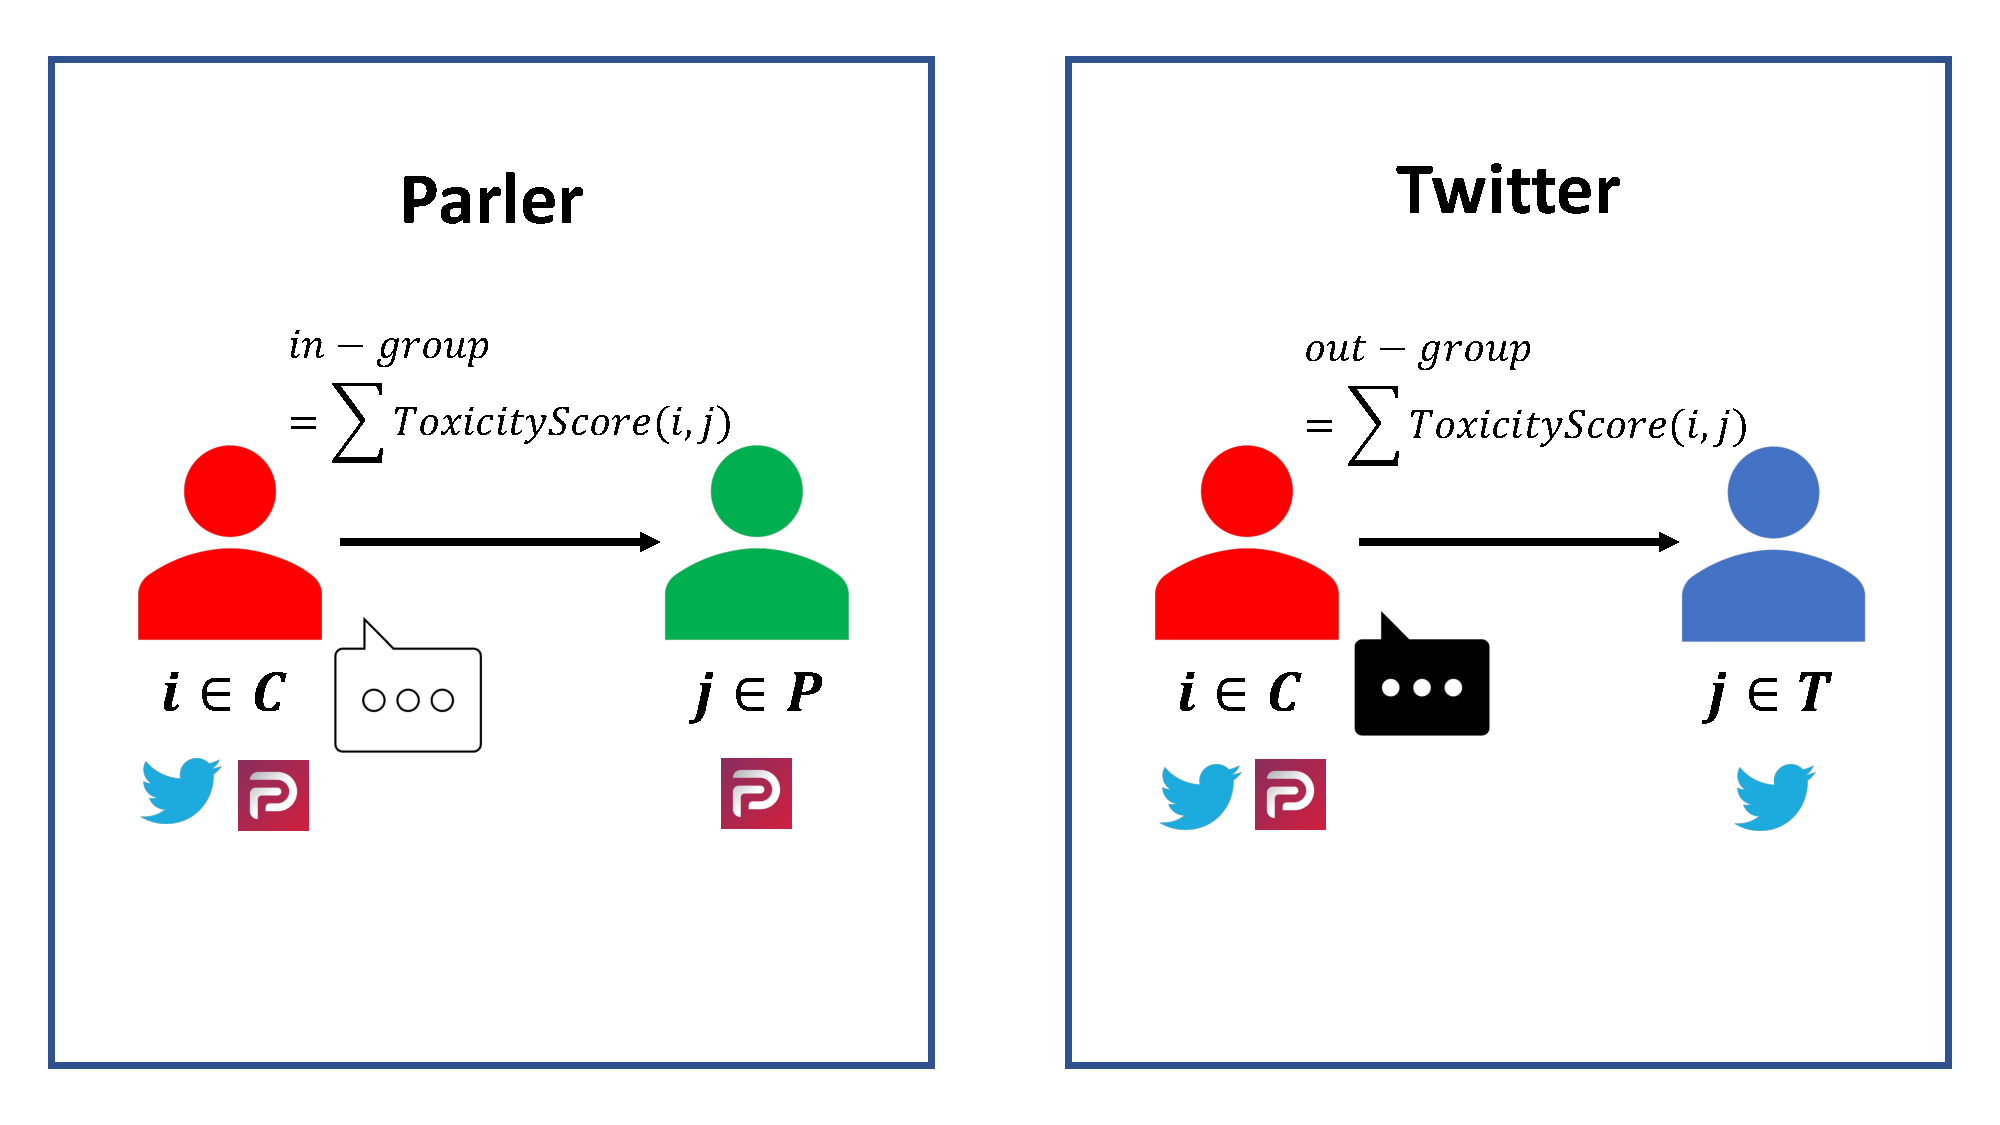
\includegraphics[scale=0.3]{figure/within-platform-v4.pdf}
    \caption{The illustrated explanation of in-/out-group code-switching.
    % within-platform code-switching. 
    The red user figure ($i \in C$) represents a cross-platform 
    user while the green human figure ($i \in P$) represents a user in 
    Parler and the blue human figure ($i \in T$) represents a user in Twitter. 
    The comparison of user level in-/out-group toxicity score was measured 
    between the average of in-group communication toxicity and out-group communication toxicity.}
    \label{fig:within-platform}
\end{figure}

\begin{equation} 
    \centering
    Toxicity\:Score(A,B) = \frac{\displaystyle\sum_{{i} \in sm(A), {j} \in sm(B)} f_{perspective}({i},{j})}{|sm(A)| \times |sm(B)|}  
    \label{eq: perspective}
    \vspace{1mm}
  \end{equation} 

Assuming that cross-platform users migrated to Parler because of
their dissatisfaction with Twitter's misinformation policy and 
their support for Trump, we hypothesized that Twitter is
an ideologically heterogeneous communication space while Parler is
an ideologically homogenous communication space.
With these assumption, in-group communication is defined as
the communication between cross-platform users and other users in Parler
while out-group communication is defined as the communication between
cross-platform users and other users in Twitter.

In answering RQ2, we explored cross-platform users' language 
when they talked to different user groups across platforms. 
Since we did not change the topic of conversation (voter fraud) 
in both Twitter and Parler, this analysis fell under 
Hudson's situational code-switching \cite{hudson_1996}. 
The situation changed in this analysis was which group of users 
that cross-platform users are talking to. 
We identified two possible communication situations 
and this is illustrated in Figure \ref{fig:within-platform} 
and how it is derived in equation \ref{eq: perspective}. 
In the equation \ref{eq: perspective}, \emph{sm(A)} and \emph{sm(B)} 
represent the user group of A and B. when those are plugged 
in the equation like \emph{ToxicityScore(A, B)}, 
it specifies the direction of the message: from the user group A to B. 
We derived the toxicity by averaging the scores from Perspective API. 
Coupling with Figure \ref{fig:within-platform}, 
 code-switching is best represented
\emph{ToxicityScore(C, T)} and \emph{ToxicityScore(C, P)}

\subsection{Statistically over-represented words} \label{sec:statistical}

\begin{equation}
 \begin{aligned}
   \delta_{w}^{(i-j)} = \log \frac{y_{w}^{i}+a_{w}}{n^{i}+a_{0}-y_{w}^{i}-a_{w}} \\
   - \log \frac{y_{w}^{j}+a_{w}}{n^{j}+a_{0}-y_{w}^{j}-a_{w}}
 \end{aligned}
 \label{eq: log-odds ratio}
 \vspace{2mm}
\end{equation}

In order to answer RQ 3, where we address different word choice of users 
who are highly engaged with others in the discussion of voter fraud, 
we used log-odds ratio with informative Dirichlet priors \cite{monroe2008fightin}. 
Log-odds ratio with informative Dirichlet estimates the log-odds ratio 
of each word $w$ between two corpora $i$ and $j$ given the prior frequencies 
obtained from corpus $a$. When $n^i$ is the size of corpus $i$, $y_w^i$ 
is the frequency of word $w$ in corpus $i$ , $a_0$ is the size of corpus, 
and $a_w$ is the frequency of the word $w$ in the corpus \cite{kwak2020systematic}. 
This approach reduced a disproportionate number of word samples by 
considering ratios and smoothed Dirichlet prior on words in the vocabulary. 
We calculated log-odds ratio of the words used by cross-platform users 
when they are in in-group communication situation compared to out-group communication situation 
similar to the research that examines distinctive discourse communities \cite{park2023quantitative}.

\section{Results}

\subsection{RQ 1. Network analysis} \label{sec:network}

\begin{figure}[htp]
  \centering
  \includegraphics[width=12cm]{figure/RQ3rr_shape.pdf}
  \caption{The network of top 20 degree centrality cross-platform users.
  The color represents the user membership 
  (Red circle: the cross-platform users, Blue cross: the users only found in Twitter.) 
  The size represents the degree centrality and for the layout, we used the spring layout from Python library NetworkX was used to visualize the network.} 
  \label{fig: network analysis}
\end{figure}

We visualized the network of the top 20 degree centrality cross-platform users to describe different degrees of homophily in Figure \ref{fig: network analysis}. However, due to the sheer difference in the size of data from Parler and Twitter, the figure mostly describe the communication patterns of the cross-platform users (in-group) and only-Twitter users (out-group).
The degree centrality was calculated based on the whole data of our observation period. As a result, the top 20 degree centrality cross-platform users network included 1,833 nodes and 6,688 edges. At a glance, Figure \ref{fig: network analysis} suggests that cross-platform users (red) who were found to have high degree centrality were connected to the users who only used Twitter (blue). In addition, cross-platform users (red) sized smaller than big nodes were connected and located inside of the cluster, connected with many cross-platform users (red). After we identified their distinctive communication feature, we calculated the different degree of EI-index for the users. 

\begin{table}[]
  \resizebox{\textwidth}{!}{%
  \begin{tabular}{c|c|c||c|c|c}
  Rank    & Degree centrality & EI-index    & Rank & Degree centrality & EI-index \\ \hline
  User 1  & 0.4485       & 0.8299 & User 21   & 0.0054   & -1                \\
  User 2  & 0.3362       & 0.7310 & User 22   & 0.0049   & -1                \\
  User 3  & 0.2125       & 0.7385 & User 23   & 0.0049   & -1                \\
  User 4  & 0.1090       & 0.7100 & User 24   & 0.0049   & -1                 \\
  User 5  & 0.0670       & 0.6910 & User 25   & 0.0044   & -1                  \\
  User 6  & 0.0310       & 0.7544 & User 26   & 0.0044   & -1                 \\
  User 7  & 0.0288       & 0.3962 & User 27   & 0.0038   & 0.4286             \\
  User 8  & 0.0218       & 0.4500 & User 28   & 0.0038   & -1                   \\
  User 9  & 0.0207       & 0.2632 & User 29   & 0.0038   & -1                  \\
  User 10 & 0.0196       & 0.3333 & User 30   & 0.0038   & -1                  \\
  User 11 & 0.0163       & 0.6667 & User 31   & 0.0038   & -1                  \\
  User 12 & 0.0158       & 0.6552 & User 32   & 0.0033   & -1                  \\
  User 13 & 0.0131       & 0.8333 & User 33   & 0.0033   & -1                   \\
  User 14 & 0.0131       & 0.5000 & User 34   & 0.0033   & -1                   \\
  User 15 & 0.0120       & 0.8182 & User 35   & 0.0033   & -1                  \\
  User 16 & 0.0093       & 0.4118 & User 36   & 0.0033   & -1                   \\
  User 17 & 0.0087       & -1 & User 37       & 0.0027   & -1                      \\
  User 18 & 0.0065       & -1 & User 38       & 0.0027   & -1                        \\
  User 19 & 0.0060       & 0.4545 & User 39   & 0.0027   & -1                   \\
  User 20 & 0.0055       & 0.2000   & User 40 & 0.0021   & -1                          
  \end{tabular}%
  }
\caption{The EI-index score of top 40 degree centrality cross-platform users}
  % \vspace{-2mm}
\label{tab:top40}
\end{table}
  
We present Table \ref{tab:top40} for detailed information about degree centrality and EI-index. Among the top 40 degree centrality users, the top 16 cross-platform users showed higher heterophily indicated by larger EI-index score. The highest EI-index score was 0.8299. On the other hand, most of the cross-platform users who were ranked out of 21 showed a complete homophily indicated by the EI-index score of -1. 
To answer RQ1, we observed different patterns of communication networks among cross-platform users' in-group and out-group communication. The cross-platform users with high degree centrality (top 20) showed high heterophily (favoring out-group communication), whereas lower degree centrality users (from top 21 to 40) showed high homophily (favoring in-group communication).

\subsection{RQ 2. In-/out-group code-switching} \label{sec:RQ2}

\begin{figure}[htp]
  \centering
  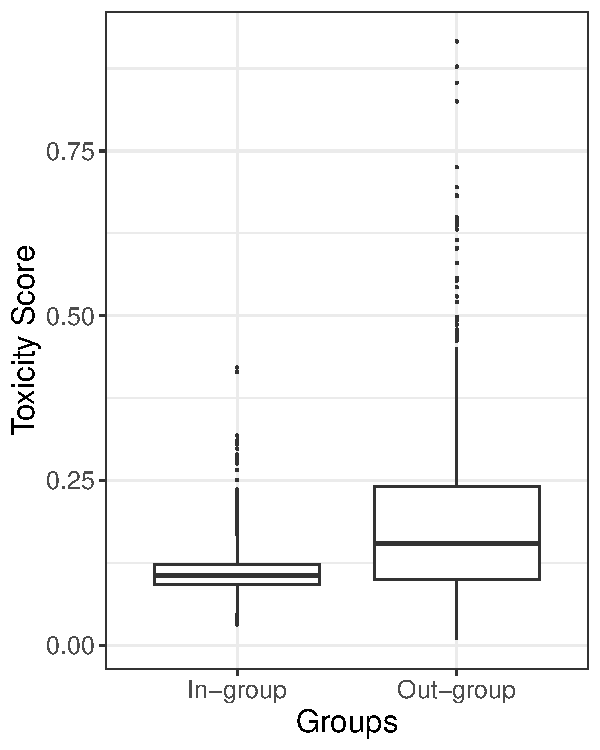
\includegraphics[width=7.5cm]{figure/toxicity_boxplot.pdf}
  \caption{The distribution of in-group and out-group toxicity scores of cross-platform users.} 
  \label{fig:RQ2_code-switching}
\end{figure}

In this section, we aim to address RQ 2 which we designed to measure situational code-switching.
For this analysis, we excluded cross-platform users (1) who did not mention other users at all 
or (2) who mentioned only either in-group users or out-group users to observe code-switching behavior. 
This is to make sure we compare changes between in-group and out-group communication. 
If cross-platform users only talked to cross-platform users (in-group), then we cannot quantitatively measure 
how this user changed the toxicity in their language when they talk to the out-group members.
We found that on average, cross-platform users exhibited more toxic language when they communicated 
with out-group members than when they communicated with in-group members. 
When cross-platform users engage in in-group communication they showed a 0.1121 toxicity score on average, 
whereas their out-group communication showed an average score of 0.1840. 
The detail of the difference between in-/out-group toxicity score is presented in Figure \ref{fig:RQ2_code-switching}. 
To delve into the relationship between in-group and out-group communication toxicity, 
we first used a t-test to compare different toxicity levels of in-group and out-group communication. 
The result in Figure \ref{fig:RQ2_code-switching} shows that the means of the two groups 
are significantly different ($t = -18.89, df = 1,347, p \leq 0.05$). 

Next, we developed an Ordinary Least Square (OLS) regression model to predict toxic level of out-group communication with three variables: (1) the toxicity score when cross-platform users engage in in-group communication, (2) the number of communication the cross-platform users talked to out-group members, and (3) the number of communication the cross-platform users talked to in-group members. The result of OLS only proved that the in-group toxicity shows correlationship between out-group toxicity regardless of the number of communication the cross-platform users talked out-group members ($p=0.408$) and the number of communication the cross-platform users talked to in-group members ($p=0.812$). We are informed that out-group communication toxicity is positively associated with in-group toxic level in Parler ($coef: 0.9389, p \leq 0.05$). 
In sum, to answer RQ2, we found that the out-group communication toxicity level of cross-platform users is higher than the in-group communication toxicity level of cross-platform users. For the relationship between in-group and out-group toxicity, we found that the toxicity level of out-group communication is positively associated with that of in-group communication. Furthermore, we found that the number of in-group or out-group communication contents did not have a significant impact on out-group communication toxicity.

\subsection{RQ 3. Over-represented words in in-group and out-group communication} \label{sec:RQ3}

\begin{figure}[htp]
  \centering
  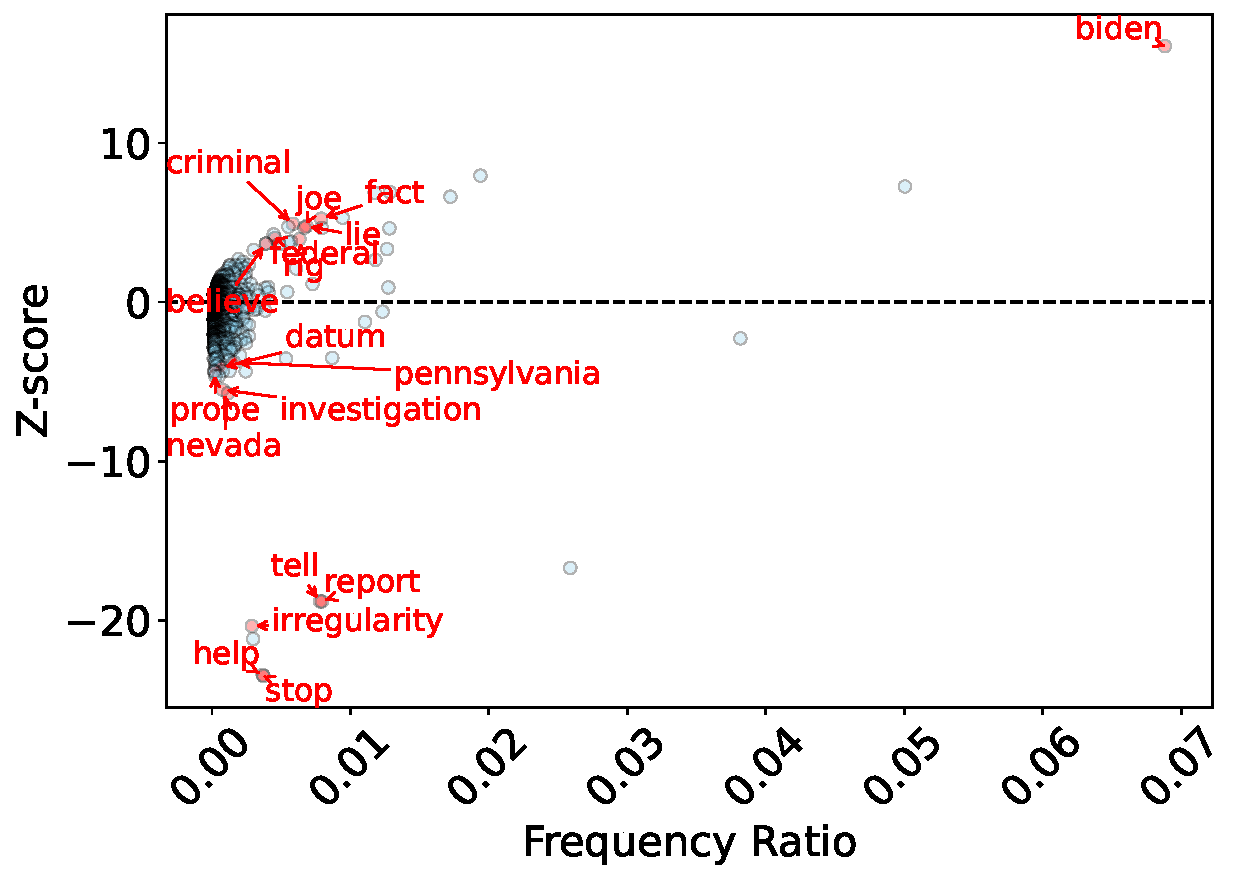
\includegraphics[scale=0.5]{figure/RQ4rr-parler-twitter-comparison-new.pdf}
  \caption{Log-odds ratios with informative Dirichlet prior result}
  \label{fig: log-odds ratios}
\end{figure}

In order to answer RQ 3, we used log-odds ratio \cite{monroe2008fightin} to find over-represented words used by cross-platform users on an in-group dominated platform (i.e., Parler) and an out-group dominated platform (i.e., Twitter). 
Figure \ref{fig: log-odds ratios} visualizes the words being used by cross-platform users in the context of frequency ratio and the Z-score. The positive Z-score suggests the word is over-used on Twitter by cross-platform users; on the other hand, the negative Z-score indicates the word is over-used on Parler. The x-axis represents the frequency of the word in the entire dataset.

We zoomed in to focus on the words in the range from 0.000 to 0.010 on the x-axis, which is where the most of words appeared. This resulted in excluding the words, \textit{``fraud''} (Z-score: -2.2780, Frequency ratio: 0.045), \textit{``election''} (Z-score: 7.2733, Frequency ratio: 0.0427), \textit{``voter''} (Z-score: -16.7041, Frequency ratio: 0.0314), \textit{``vote''} (Z-score: -0.5983, Frequency ratio: 0.0184), \textit{``trump''} (Z-score: -1.2380, Frequency ratio: 0.0162), \textit{``ballot''} (Z-score: -3.5029, Frequency ratio: 0.0121) from the Figure \ref{fig: log-odds ratios}.
Since the keywords we used for data collection already included topical words about the election (See footnote \footref{footnote1} on page \pageref{footnote1}), election-related keywords appeared frequently throughout the dataset. We also excluded these election-related keywords because  they do not carry meaningful information about the difference in language use of the cross-platform users.

Table \ref{tab:z-score} show top 20 words which are most statistically over-used on Twitter and Parler by cross-platform users.
We found that \textit{``joe''} and \textit{``biden''} were more frequently used on Twitter by cross-platform users. 
We are visually informed in Figure \ref{fig: log-odds ratios} that the word \textit{``irregularity''}, \textit{``help''}, \textit{``stop''}, \textit{``report''}, and \textit{``tell''} are more frequently used on Parler compared to Twitter by cross-platform users. 
The word \textit{``stop''} being over-represented on Parler could be in reference to the slogans, \textit{``Stop the Steal''} and \textit{``Stop the count''} 
that were used by Trump supporters to protest against the election result.
The words, \textit{``help''}, \textit{``report''}, \textit{``tell''}, and \textit{``say''} that are heavily represented on Parler 
are encouraging words that are associated with the action of reporting the election fraud. The word \textit{``datum''} (data) and \textit{``irregularity''} 
could tell us what the cross-platform users want to find from the election.

On Twitter, the words \textit{``fact''} and \textit{``lie''} were frequently used by cross-platform users. 
This might be because the discourse around election fraud on Twitter was about the fact-checking of the election fraud claims. 
The word \textit{``believe''} implies that the election fraud claims are a psychological state where in-group members believe the politician's messages 
are truthful, while the opposing out-group believes the messages are deceptive \cite{ehrlich2015politics, clementson2018truth}. 
On the other hand, the words \textit{``probe''} and \textit{``investigation''} are more frequently used on Parler. 
This may indicate that the discourse around voter fraud was about investigating the election fraud claims, and these are more specific action words 
toward the election fraud claims. Similarly, the words \textit{``nevada''} and \textit{``pennsylvania''} (Z-score: -3.7827 and ranked lowest 23) 
could be connected to the place where \textit{``investigation''} should take place. 
Action-related words such as \textit{``report''} and \textit{``tell''} could be the way to substantiate their voter fraud claims. 
However, we still found some keywords related to voter fraud claims, such as claiming the election is \textit{``rig''}-ged and 
hose who orchestrated the election fraud are \textit{``criminal''}-s on Twitter. The word \textit{``federal''} might be used 
to refer to the federal government that is responsible for the election. 
This suggests that the discourse around voter fraud were not only prevalent on Parler but also on Twitter.

\begin{table}[h]
  \resizebox{\textwidth}{!}{%
  \begin{tabular}{c|c|c||c|c|c}
  Word         & Z-score     & Frequency ratio & Word          & Z-score      & Frequency ratio \\ \hline
  biden        & 16.0956 & 0.0098     & stop          & -23.5147 & 0.0025     \\
  president    & 7.9568 & 0.0074     & help          & -23.4308 & 0.0014     \\
  election     & 7.2733 & 0.0427     & us            & -21.1774 & 0.0008     \\
  lose         & 6.9193 & 0.0019     & irregularity  & -20.3643 & 0.0004     \\
  must         & 6.8829 & 0.0036     & report        & -18.8175 & 0.0039     \\
  concede      & 6.6286 & 0.0014     & tell          & -18.8153 & 0.0047     \\
  go           & 5.3081 & 0.0084     & voter         & -16.7041 & 0.0314     \\
  fact         & 5.2464 & 0.0013     & nevada        & -5.7350 & 0.0009     \\
  criminal     & 4.9256 & 0.0017     & investigation & -5.5063 & 0.0011     \\
  lie          & 4.7752 & 0.0017     & congress      & -4.6457 & 0.0003     \\
  involve      & 4.7435 & 0.0011     & continue      & -4.6382 & 0.0007     \\
  joe          & 4.6861 & 0.0030     & registration  & -4.4005 & 0.0003     \\
  know         & 4.6632 & 0.0068     & probe         & -4.3674 & 0.0001     \\
  donald       & 4.6394 & 0.0011     & via           & -4.3502 & 0.0020     \\
  everyone     & 4.2524 & 0.0013     & allege        & -4.3394 & 0.0009     \\
  federal      & 4.0203 & 0.0016     & law           & -4.3287 & 0.0019     \\
  rig          & 3.9557 & 0.0072     & mayor         & -4.3035 & 0.0001     \\
  deep         & 3.8156 & 0.0010     & datum         & -4.1127 & 0.0007     \\
  overwhelming & 3.7838 & 0.0004     & committee     & -4.0191 & 0.0002     \\
  believe      & 3.6824 & 0.0031     & group         & -3.8986 & 0.0004    
  \end{tabular}%
  }
\caption{Top 20 Z-score words and lowest 20 Z-score words by cross-platform users and their frequency ratio}
\label{tab:z-score}
\end{table}


\section{6. Discussion}

In this study, we explored the network and the toxicity of the language of cross-platform users who were engaged in voter fraud claims during the 2020 U.S. presidential election on two ideologically distinctive social media platforms. 
The phenomenon where the users who have Twitter accounts decided to use Parler and created a space for like-minded people to communicate provided a rare opportunity to examine how people in the real world communicate differently based on the political climate of the platform they are on. From \nameref{sec:network}, we found that cross-platform users demonstrate varying levels of homophily in their connections with other users. The cross-platfrom users with high degree centrality were more likely to communicate with out-group members (heterophily), whereas the cross-platfrom users with low degree centrality were more likely to communicate with in-group members (homophily). This finding suggests that the cross-platform users exhibited different in-group and out-group communication patterns.

From \nameref{sec:RQ2}, we found that cross-platform users used more toxic language in out-group communication than in-group
communication. This finding is consistent with Sumner's theory that out-group relationships tend to be more hostile than 
in-group relationships \cite{sumner1906folkways}. 
Extending social identity theory, we argue that cross-platform users were more likely to be in peace on Parler, 
as they found Parler is a safe space for like-minded people, and thus formed an echo chamber of in-group communication network
\cite{zannettou2018gab}. On the other hand, for cross-platform users, Twitter can be considered as an ideologically 
heterogeneous communication space. Since many cross-platform users departed Twitter for political reasons, 
it is fair to say Twitter is, from their point of view, a more diverse out-group dominated community. 
This pattern is consistent with Cinelli et al.'s findings where they argued 
YouTube users use inappropriate, violent, or hateful language when they argue within their opponents' community \cite{cinelli2021dynamics}.
With the t-test, we also found that out-group toxicity is statistically different from in-group toxicity and on average, 
in-group toxicity was lower than out-group toxicity. 
Lastly, in answering \nameref{sec:RQ3}, we found that the cross-platform users used different words and 
thus created different discourses on Twitter and Parler. We argue that participating within an ideologically 
congruent communication space (Parler) and an ideologically heterogeneous communication space (Twitter) 
may have influenced the choice of language. This finding adds to An et al.'s argument 
that politically homogeneous and heterogenous environments allow for differentiated accounts of behavior \cite{an2019political}. 
Differences in discourse on Parler and Twitter were qualitatively varied based on politically motivated beliefs. 
On Parler, the discourse around voter fraud claims was about investigating election fraud and encouraging others 
to take action to fight against the ``rigged election.'' On the other hand, we identified ``fact'' and ``lie'' 
as frequently used words in the discourse around voter fraud claims on Twitter, indicating the discourse was more 
focused on whether or not election fraud had taken place. We argue that the findings of this study would be helpful 
to open up discussion on the role of social media platforms in the online public sphere. 
As manifested in this study, different content moderation and regulation policies of a platform not only can attract 
users with different political leanings but can also affect the types of discourse and facts shared on the platform; 
thus creating different public spheres \cite{habermas1991structural}. 

In conclusion, our study sheds light on how the collective identities of cross-platform users who seeking asylum 
for free speech were reflected in their use of toxic language on two politically distinct social media platforms. 
Contrary to prevailing notions that homogeneous communicative environment, characterized as echo chambers, 
may encourage users to engage in more extreme discourse and lead them use more toxic language, our findings suggest 
the opposite pattern.
Specifically, conservative users participating in discussions on voter fraud on Twitter, a platform that is 
more diverse and more liberal than Parler, exhibited more toxic language use than they did on Parler. 
This increased hostility towards those holding different viewpoints could serve as a means to reinforce their 
collective in-group identity. 

Our findings diverge from certain prior studies, such as Zannettou et al., 
which suggests that a less strict community guideline that uphold free speech to an extreme degree fosters 
a toxic culture in an ideologically homogeneous communication space \cite{zannettou2018gab}. In contrast, our study suggests that toxic discourse find a more fertile ground in ideologically heterogeneous communication spaces, 
where individuals can target out-group members within the network. Our findings of prevalent toxic language exhibition 
in ideologically heterogeneous communication space is not new. Similar to our findings, one study examined the changes 
of toxic language use after the users were deplatformed from Twitter and migrated to alternative social media called ``Gettr.''
This study revealed that the matched users were more toxic in Twitter \cite{meakacher2023}. 
Likewise, this counterintuitive finding challenges conventional assumptions about the relationship between echo chambers, 
toxic language, and the social media platform's guidelines for free speech. 

Before concluding this study, however, several limitations should be noted. 
First, although studies on user migration attempted to classify the usernames presumably owned by 
the same user \cite{kumar2011understanding} we do not have gold standard data. 
It is hard to know the true positives and true negatives because of practical limitations that the researchers 
cannot interview all individual users by asking for their usernames. 
To address this limitation, we used Levenshtein distance (threshold of 0.90) \cite{levenshtein1966binary} 
to identify similar usernames in Parler and Twitter. This more ``greedy approach'' resulted in finding more 
matching usernames and increased our data size from N=9,371 (with the case-insensitive username matching) 
to N=38,798. Our approach for username matching, although not perfect, has led us to include possible usernames 
that might have been missed when strictly using the exact matching.

Second limitation of this study is our narrow definition of in-group and out-group. 
Our definition of in-group focuses on how cross-platform users (defined by the matching usernames) 
were active on certain platforms. We did not make use of other socio-demographical factors such as gender, 
address, age, race, and political ideology that can be found in user profiles. Therefore, it is possible 
our definition of in-group and out-group based on the platform use may not be the same as the in-group and out-group 
distinction based on the users' political orientation.
Third, although Parler and Twitter share similar affordances \cite{bucher2018affordances} such as likes (in Parler, votes) 
and retweets (in Parler, echoes), there still are substantial differences across the platforms including 
their community guidelines \cite{m2021political}. This study was not able to test how these potential differences 
might have affected user behaviors. In addition, the size of Twitter data were significantly bigger than the size 
of Parler data, which impacted RQ 1. where most of data for network analysis was from Twitter as high degree centrality users
were more active in Twitter.

\section{7. Ethical consideration}

With respect to a method-related ethical concern, we attempted to aggregate the data by defining cross-platform users and homophilous (heterophilous) users and compared their average level of toxicity. This aggregating method was found to make users feel comfortable when researchers make use of their data \cite{dubois2020journalists} because it reduces the chance of revealing who the real person is, using specific user accounts behind. However, it is another dimension of discussion when data was deleted and made available without their collective consent. Officially Parler stopped the service after the January 6th Capitol attack \cite{m2021political}. Even though platforms have the authority to enforce terms of service, it is hard to draw a clear line \cite{blackwell2017classification} whether it is ethical to use archived data when the service is discontinued \cite{fiesler2020no}. It may beyond the platform governance, potentially have ethical implications for resurrecting deleted data for research. To understand antisocial behavior in social media, researchers found banned users' past activities and their contents, which were deleted \cite{chandrasekharan2017you}. However, using deleted Parler data for research requires a different dimensional approach because unlike banning the users in Reddit which is still in service, Parler is deleted completely. As Almuhuimedi et al. found out, there are ways to find deleted social media content and the availability of deleted social media content raises security and privacy implications \cite{almuhimedi2013tweets}. We may face questions that touch on recovering deleted content from discontinued social media services for research purposes.  
The publicly available Parler data \cite{aliapoulios2021large} we used was collected before Parler stopped the service. With this dataset, we joined it with our collected tweets using Twitter API. However, since we identified the usernames as a tool to merge two datasets, it may pose another dimension of the ethical issue of using social media data for research. The cross-platform users might have agreed on the terms of service provided by each platform. However, just because the users agreed on both terms of service, it does not automatically grant the permit to use their data by joining them. This unanswered question will lead us to think about how to use multiple social media data even though it is open to all and waiting to be used for various research. In addition, we suspect many of the users included in our analysis are already banned from Twitter. Therefore, other researchers who might want to replicate our study may find different results. 
    
\section{8. Conclusion}

We explored how users of two social media platforms used toxic language differently (cross-platform analysis) 
and how users talked to in-/out-group users. To our knowledge, there is no study empirically borrowed code-switching theory to study social media. Although our study brings a unique context (voter fraud claim during the 2020 U.S. Presidential Election), this study synthesized the code-switching behavior of the users for the first time. In addition, we discussed the ethical consideration of joining multiple social media datasets and using the deleted dataset for research. When joining multiple social media datasets, it raises an extra caution not to use personally identifiable data because users may be granted the data access to individual social media platforms but their identity may be revealed by coupling multiple datasets. We hope this study initiates the discussion around how we can make use of multiple social media datasets within the boundary of ethical use of data.

\bibliography{bibliography}
\end{document}

